
\newpage
\section{Anhang}

\subsection{Musteranmeldeformular}
\begin{figure}[H]
    \centering
    \caption{Musteranmeldeformular von der fiktiven Person Max Müller}
    \begin{adjustbox}{height=0.85\textheight, center}
        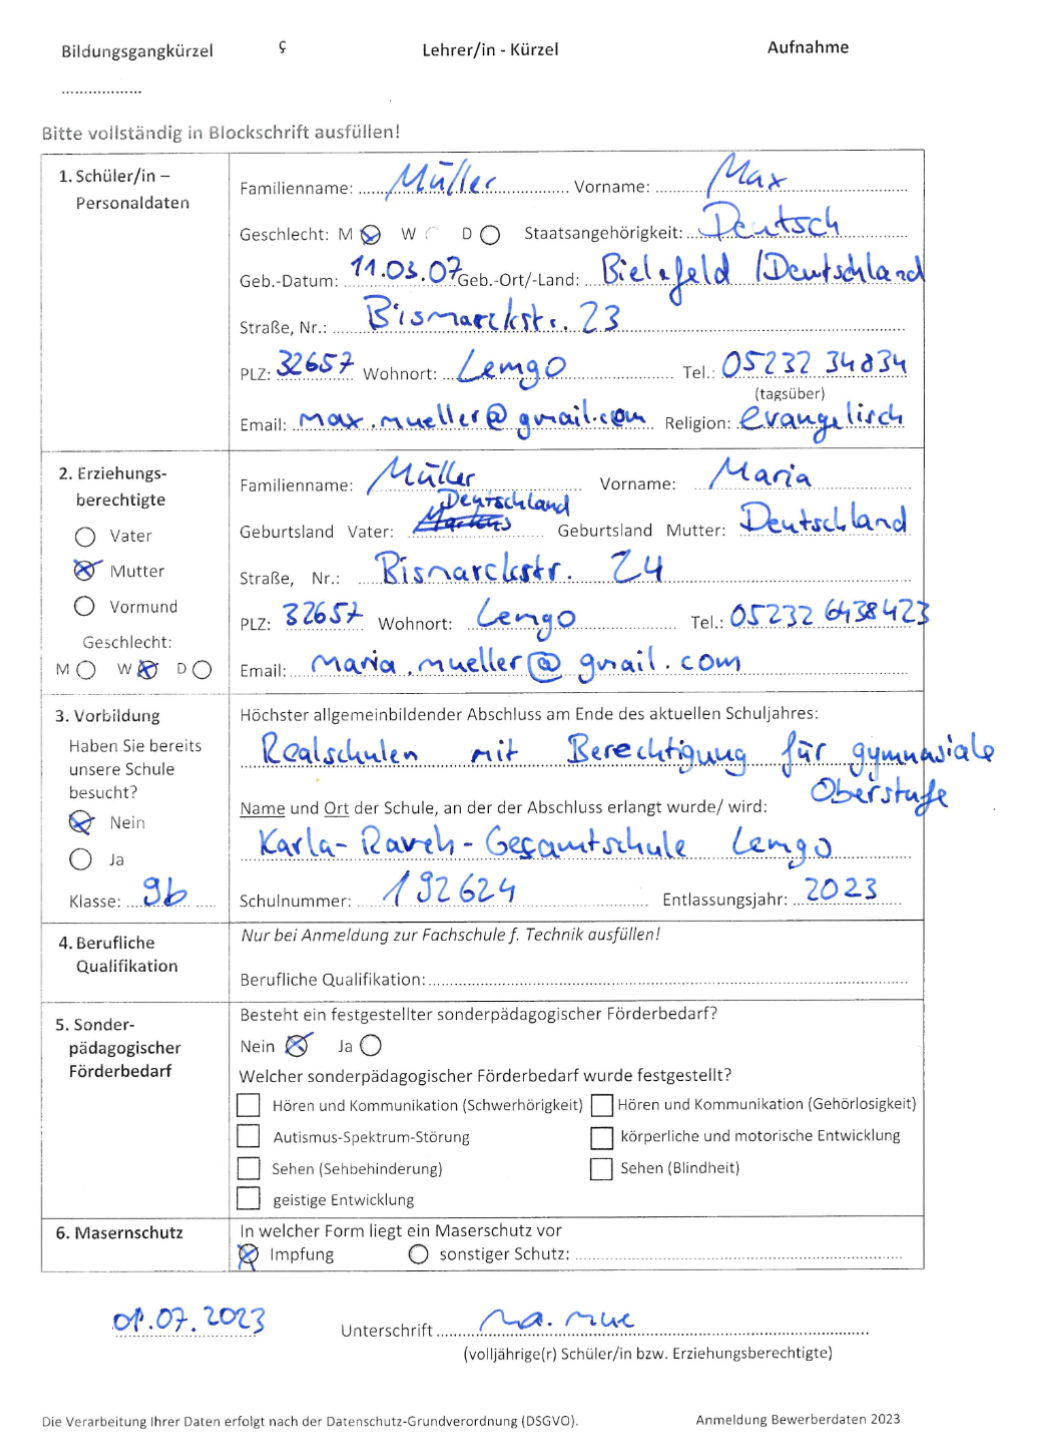
\includegraphics{bewerbungsformular1}
    \end{adjustbox}
\end{figure}

\begin{landscape}

    \begin{longtable}{p{15cm}cc}
        \caption{Your Table} \label{tab:mytable} \\
        \toprule
        Erfordernis: Der Benutzer muss... & Zugehörige Ergebnisse \\
        \midrule
            ... inkorrekte Daten identifizieren und korrigieren können. & E1, E2 \\
            ... die an ihn eingereichten Formulare korrekt übertragen können. & E5, E6 \\
            ... unzulässige Bewerbungen identifizieren können. & E9, E10 \\
            ... die Daten datenschutzkonform in die Anwendung eintragen können und über mögliche Verstöße informiert werden. & E11 \\
            ... erkennen können, wie er zum korrekten Prozess gelangt. & E12 \\
            ... bezüglich Aufnahmeentscheidungen mit den Entscheidungsträgern zusammen arbeiten können. & E7, E8 \\
            ... die Software auch bei fehlenden Daten bedienen können.  & \\
            ... Aufnahmekriterien berücksichtigen können. & \\
            ... Termine für Aufnahmeberatungsgespräche hinterlegen können. & b \\
            ... Schülerakten erzeugen können. & b \\
            ... Daten aus anderen Programmen übernehmen können. & b \\
            ... Adressrecherchen durchführen können. & b \\
            ... eine Kurzanleitung für den Einstieg abrufen können. & b \\
            ... die Software auch bei fehlenden Daten bedienen können. & b \\
            ... innerjährige Wechsel und Stufenwiederholungen erfassen können. & b \\
            ... langfristige Beurlaubungen vermerken können. & b \\
            ... auch komplizierte Bewerbungen und Sonderfälle bearbeiten können. & b \\
            ... seinen bisherigen Jargon verwenden können. & b \\
            ... die Aufgaben und Prozesse intuitiv bedienen können. & b \\
            ... eine Adressvalidierung vornehmen können. & b \\
            ... Erreichbarkeiten von Notfallkontakten erfassen können. & b \\
            ... unterschiedliche Arten von Notfallkontakten erfassen können. & b \\
            ... erkennen können, ob ein Schüler volljährig ist. & b \\
        \endfirsthead
        \toprule
        Erfordernis & Beispiel & Zugehörige Ergebnisse \\
        \midrule
        \endhead
        \bottomrule
        \endfoot
            ... Nachweise über das Sorgerecht hinterlegen können. & b \\
            ... Daten auch bei Dialogabbrüchen wiederherstellen können. & b \\
            ... ähnliche Datenabfragen aus vorherigen Formularen übernehmen können. & b \\
            ... bei Bedarf Handbücher heranziehen können. & b \\
            ... bei Bedarf Fachterminologie nachschlagen oder verstehen können. & b \\
            ... jederzeit darüber Bescheid wissen, welche Daten den Eltern und Schülern angezeigt werden. & b \\
            ... den Systemstatus jederzeit einsehen können. & b \\
            ... Bewerbungslisten in geeigneter Form exportieren können. & b \\
            ... Daten in Schulverwaltungsprogramme wie Schild exportieren können. & b \\
            ... Daten nach Excel exportieren können. & b \\
            ... Berichte anfertigen können. & b \\
            ... Anmeldezeiträume berücksichtigen. & b \\
            ... mit anderen Behörnden zusammenarbeiten können. & b \\
            ... über Änderungen an Bewerbungen regelmäßig informiert werden. & b \\
            ... zusätzliche Informationen zu einer Bewerbung hinterlegen können. & b \\
            ... Dokumente ausdrücken können. & b \\
            ... Dokumente digitalisieren und beim Datensatz hinterlegen können. & b \\
    \end{longtable}




\subsection{bildungsgang}
\begin{figure}[H]
    \centering
    \caption{Testüberschrift}
    \begin{adjustbox}{width=\linewidth, center}
        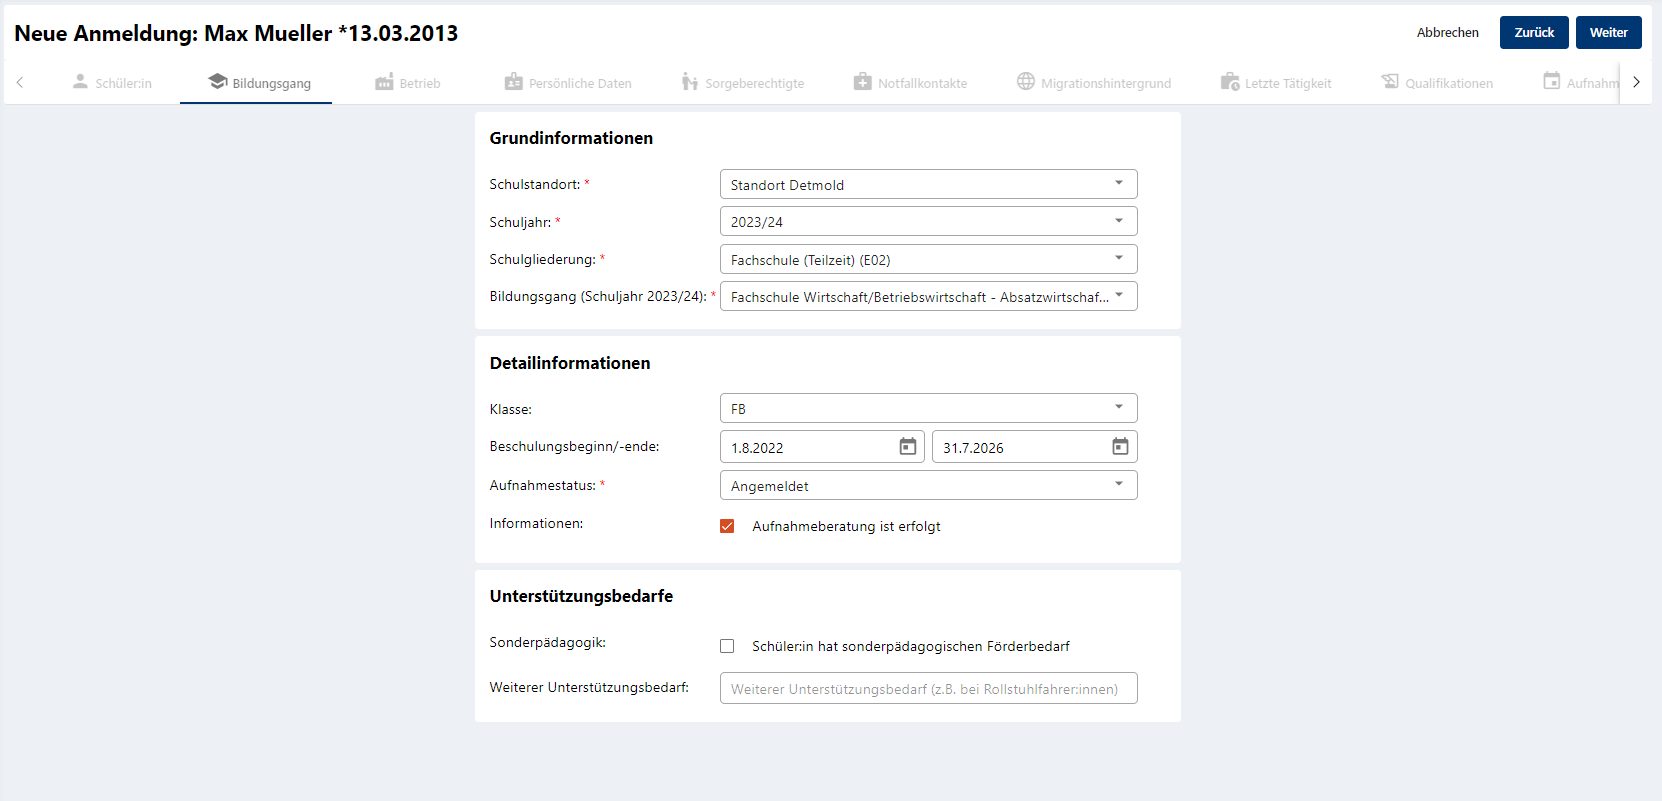
\includegraphics{bildungsgang}
    \end{adjustbox}
\end{figure}

\subsection{sorgeberechtigte-liste}
\begin{figure}[H]
    \centering
    \caption{Testüberschrift}
    \begin{adjustbox}{width=\linewidth, center}
        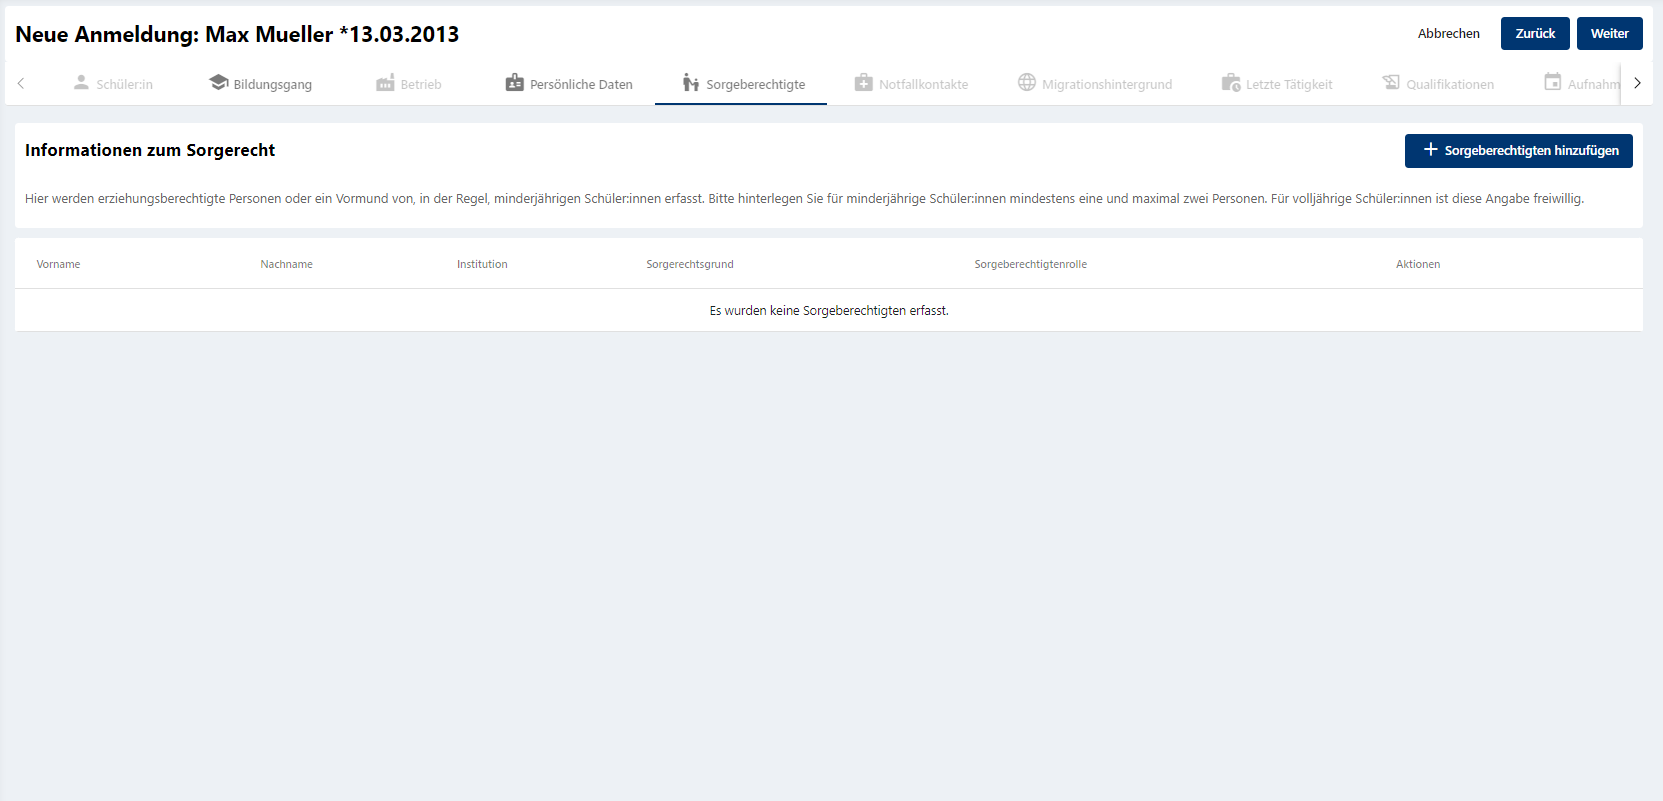
\includegraphics{sorgeberechtigte-liste}
    \end{adjustbox}
\end{figure}

\subsection{sorgeberechtigter-person}
\begin{figure}[H]
    \centering
    \caption{Testüberschrift}
    \begin{adjustbox}{width=0.5\linewidth, center}
        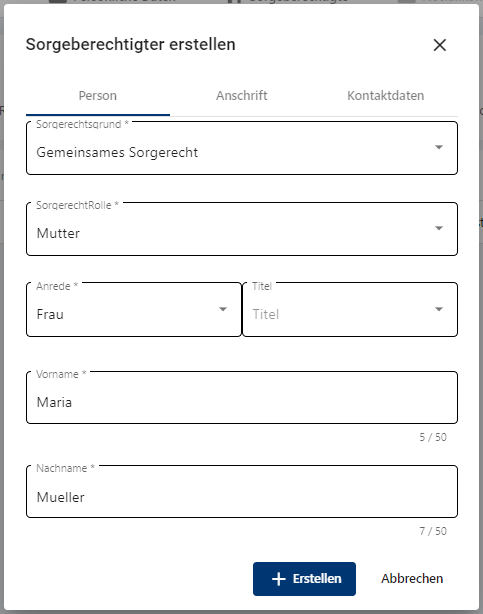
\includegraphics{sorgeberechtigter-person}
    \end{adjustbox}
\end{figure}

\subsection{sorgeberechtigter-anschrift}
\begin{figure}[H]
    \centering
    \caption{Testüberschrift}
    \begin{adjustbox}{width=0.85\linewidth, center}
        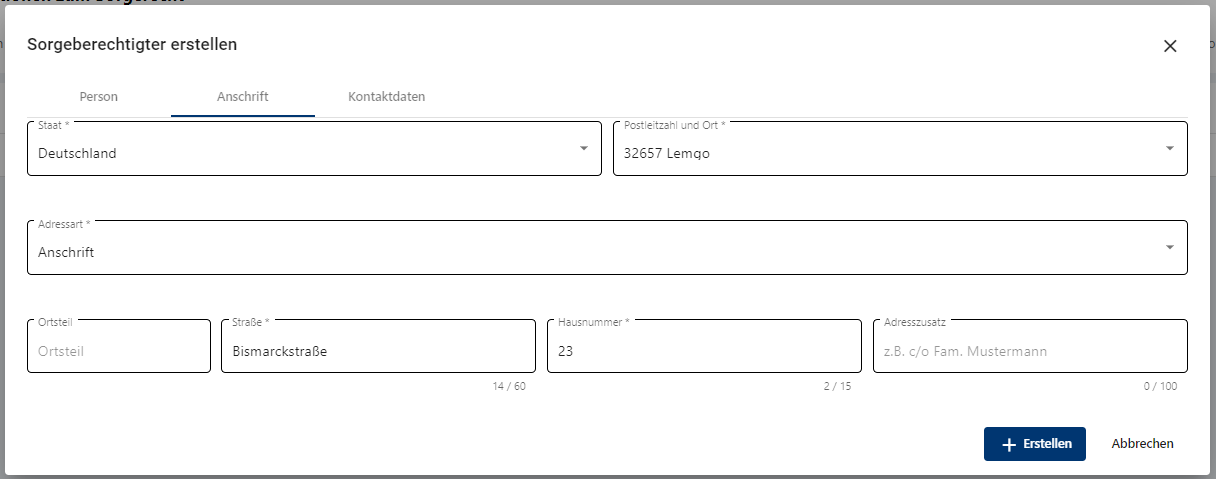
\includegraphics{sorgeberechtigter-anschrift}
    \end{adjustbox}
\end{figure}

\subsection{sorgeberechtigter-kontakt}
\begin{figure}[H]
    \centering
    \caption{Testüberschrift}
    \begin{adjustbox}{width=0.6\linewidth, center}
        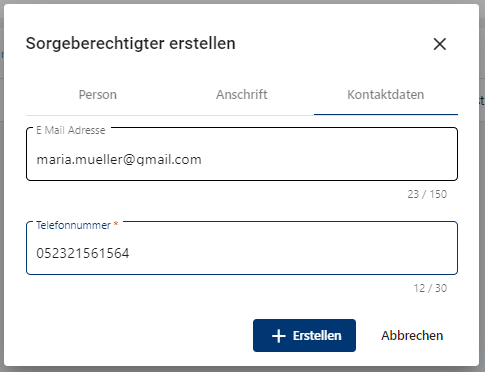
\includegraphics{sorgeberechtigter-kontakt}
    \end{adjustbox}
\end{figure}

\subsection{notfallkontakt-daten}
\begin{figure}[H]
    \centering
    \caption{Testüberschrift}
    \begin{adjustbox}{width=0.6\linewidth, center}
        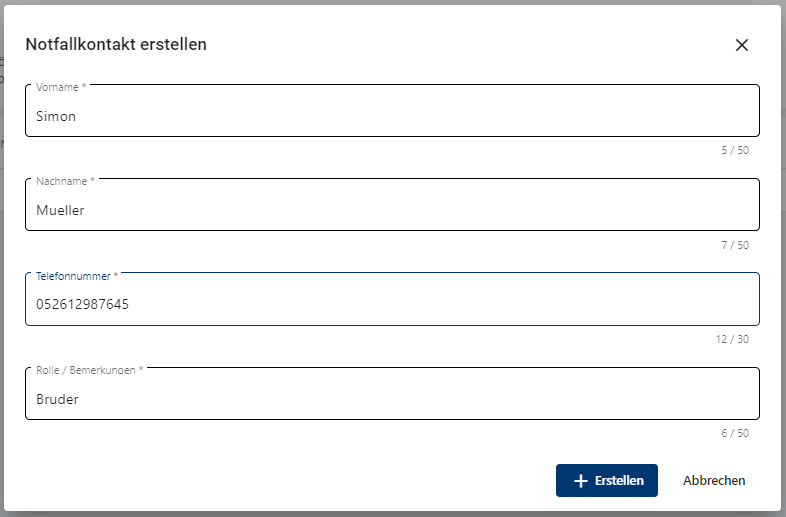
\includegraphics{notfallkontakt-daten}
    \end{adjustbox}
\end{figure}

\subsection{notfallkontakt-liste}
\begin{figure}[H]
    \centering
    \caption{Testüberschrift}
    \begin{adjustbox}{width=\linewidth, center}
        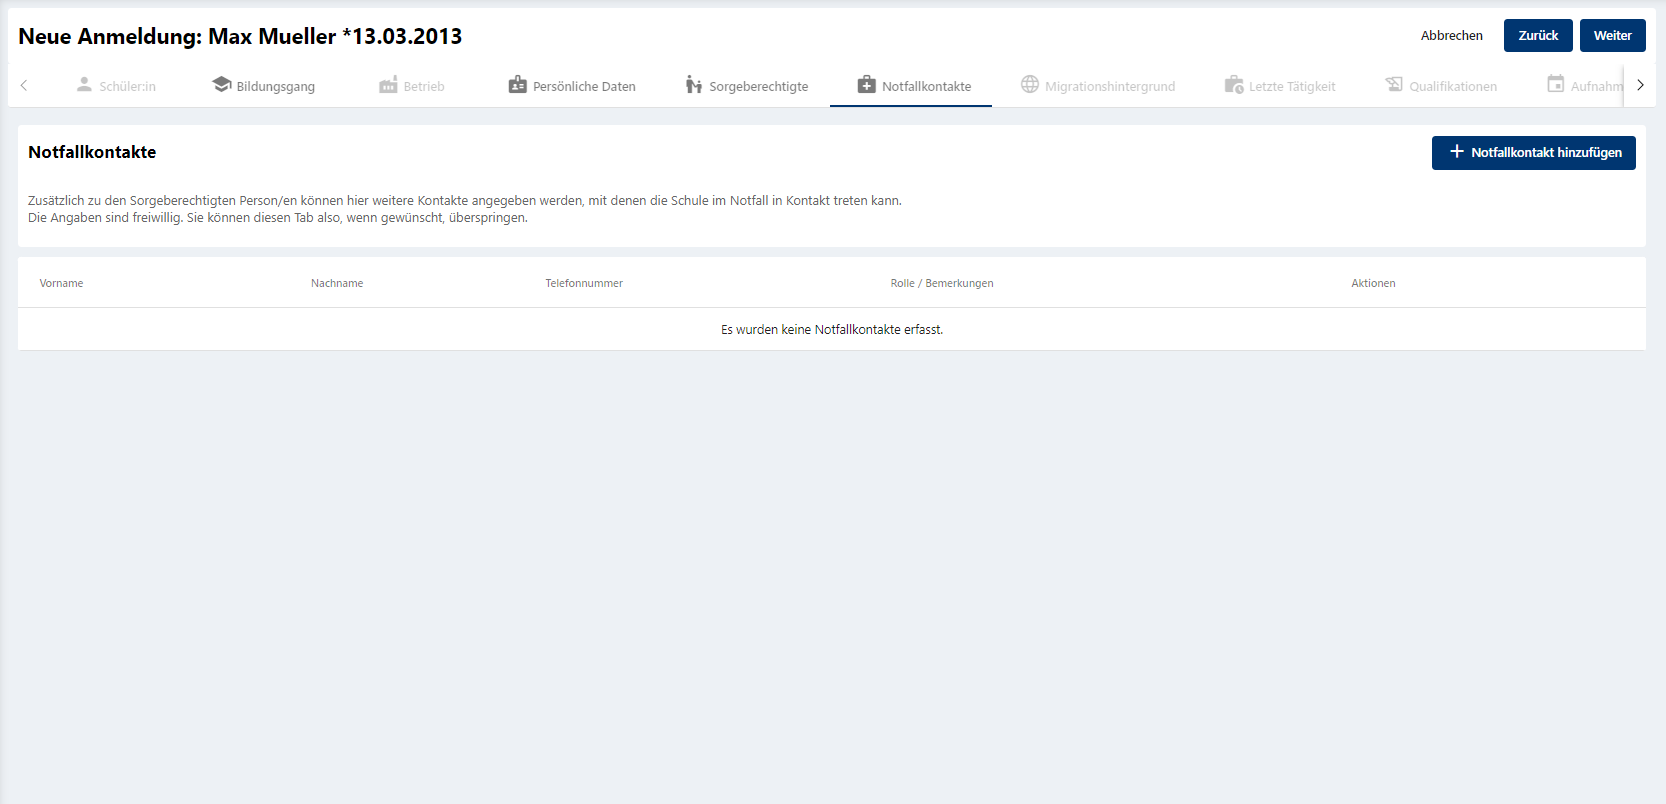
\includegraphics{notfallkontakt-liste}
    \end{adjustbox}
\end{figure}

\subsection{migrationshintergrund-liegtvor}
\begin{figure}[H]
    \centering
    \caption{Testüberschrift}
    \begin{adjustbox}{width=\linewidth, center}
        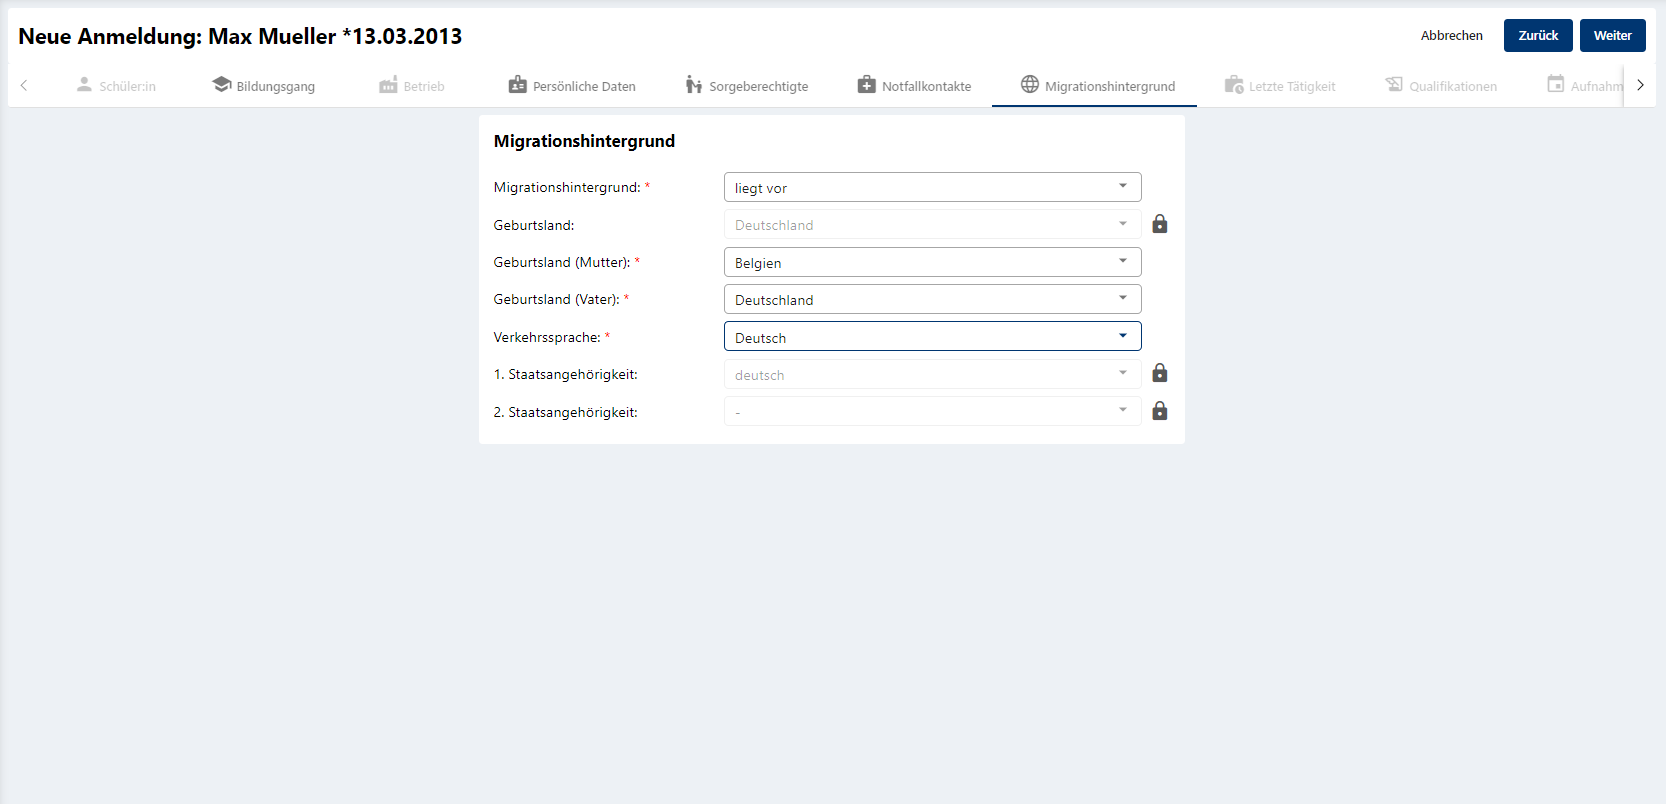
\includegraphics{migrationshintergrund-liegtvor}
    \end{adjustbox}
\end{figure}

\subsection{migrationshintergrund-liegtnichtvor}
\begin{figure}[H]
    \centering
    \caption{Testüberschrift}
    \begin{adjustbox}{width=\linewidth, center}
        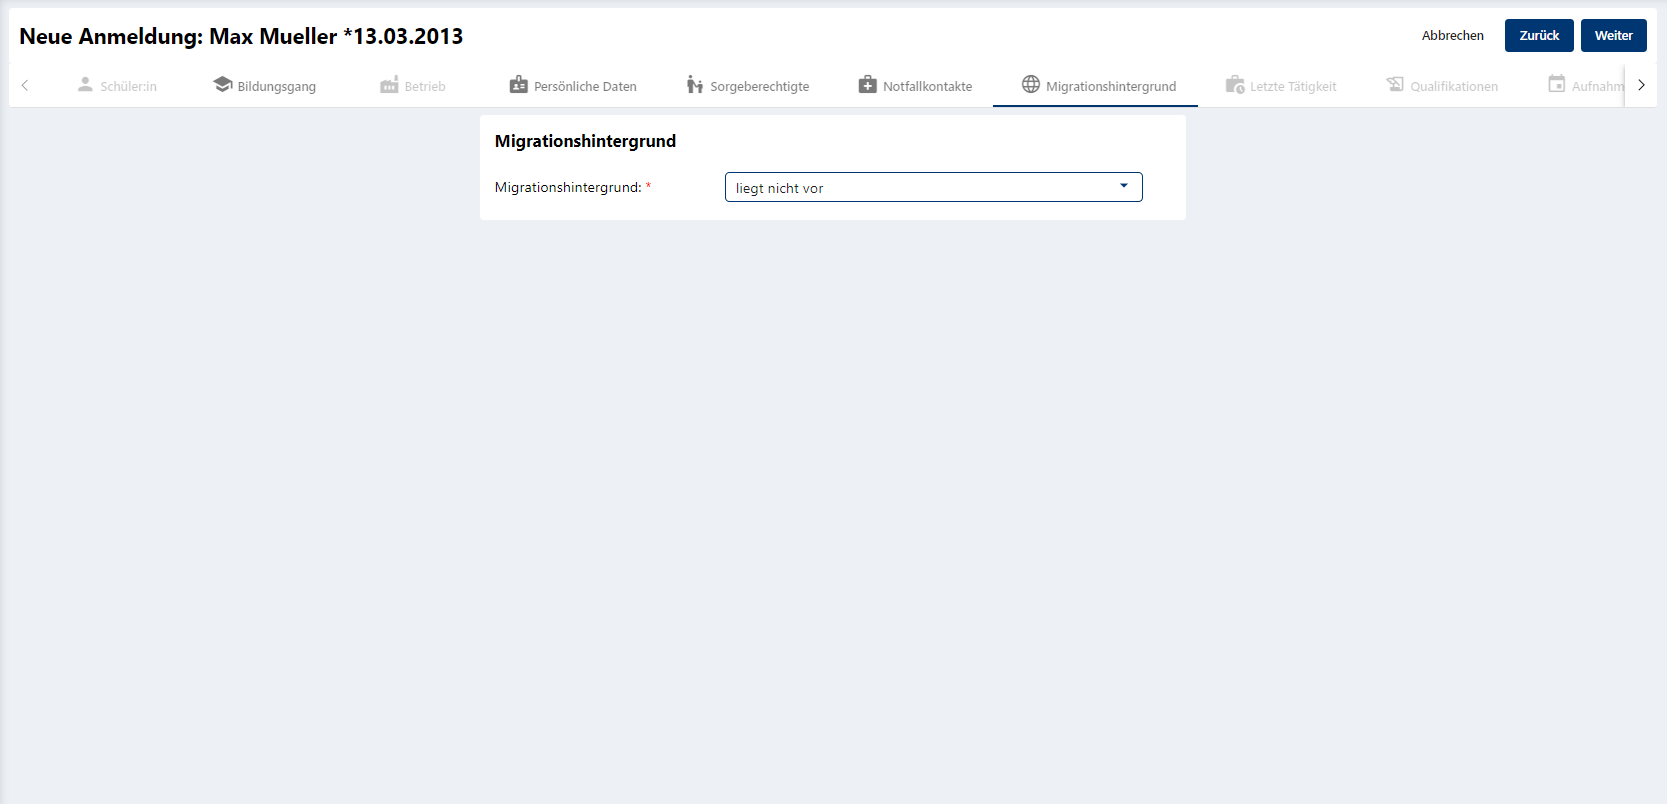
\includegraphics{migrationshintergrund-liegtnichtvor}
    \end{adjustbox}
\end{figure}

\subsection{qualifikation}
\begin{figure}[H]
    \centering
    \caption{Testüberschrift}
    \begin{adjustbox}{width=\linewidth, center}
        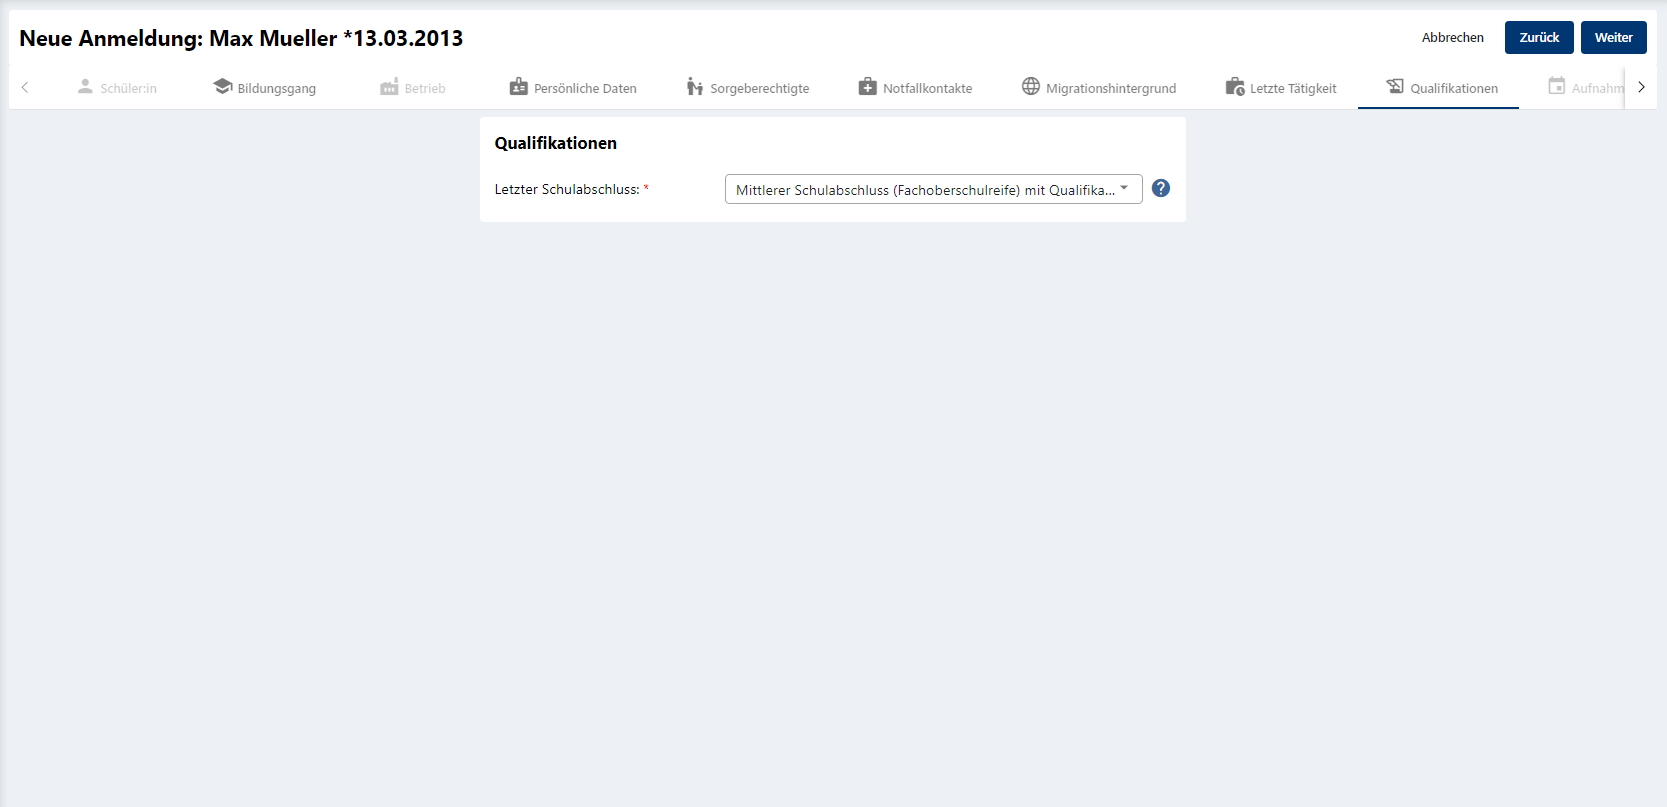
\includegraphics{qualifikation}
    \end{adjustbox}
\end{figure}

\subsection{letztetaetigkeit}
\begin{figure}[H]
    \centering
    \caption{Testüberschrift}
    \begin{adjustbox}{width=\linewidth, center}
        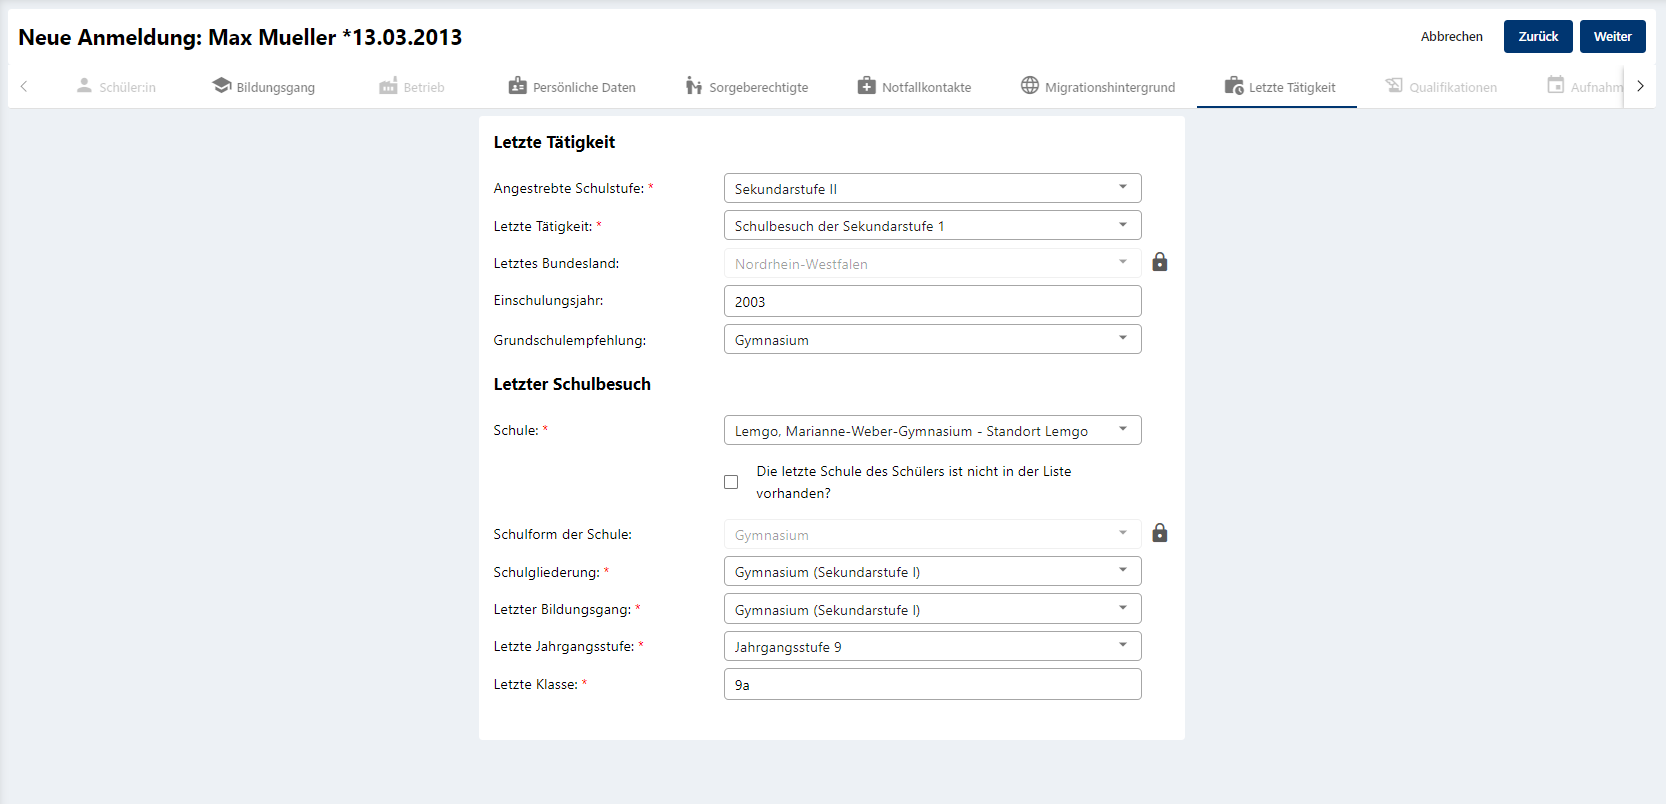
\includegraphics{letztetaetigkeit}
    \end{adjustbox}
\end{figure}

\subsection{aufnahmeberatung}
\begin{figure}[H]
    \centering
    \caption{Testüberschrift}
    \begin{adjustbox}{width=\linewidth, center}
        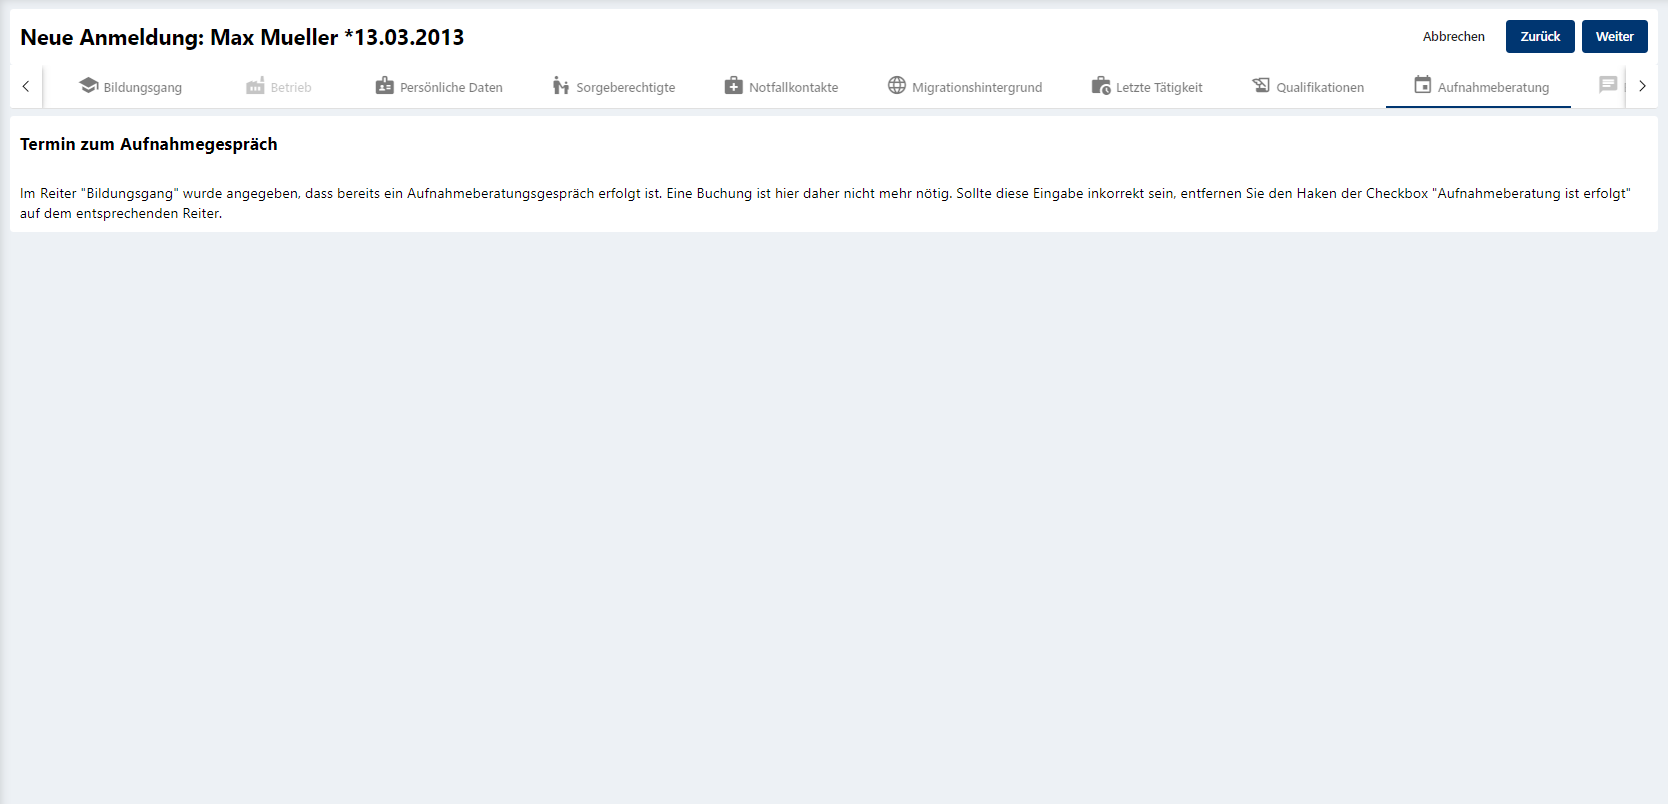
\includegraphics{aufnahmeberatung}
    \end{adjustbox}
\end{figure}

\subsection{bemerkungen}
\begin{figure}[H]
    \centering
    \caption{Testüberschrift}
    \begin{adjustbox}{width=\linewidth, center}
        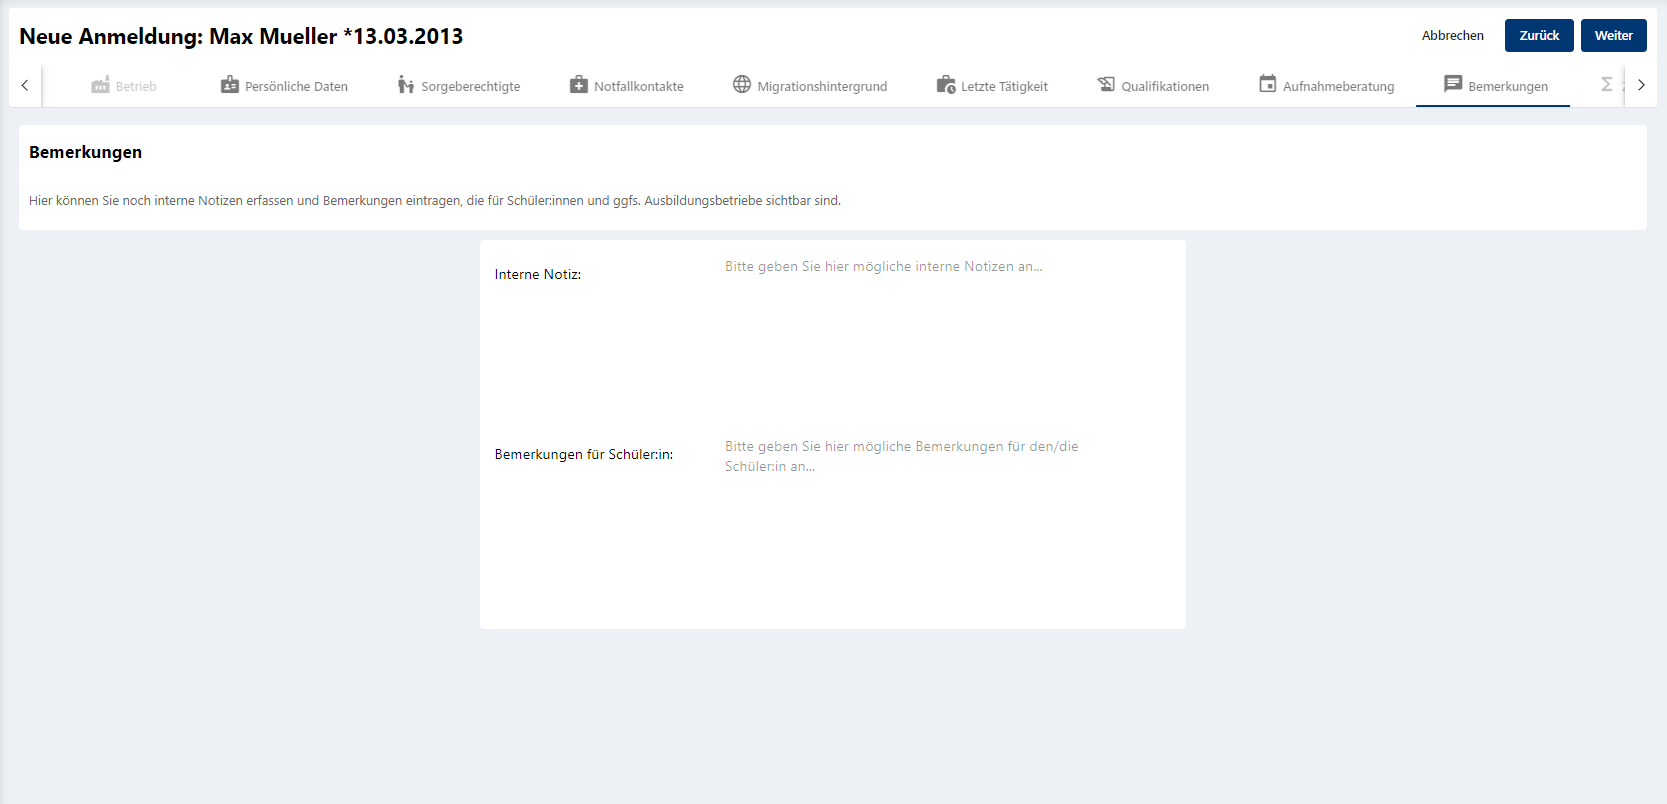
\includegraphics{bemerkungen}
    \end{adjustbox}
\end{figure}

\subsection{zusammenfassung}
\begin{figure}[H]
    \centering
    \caption{Testüberschrift}
    \begin{adjustbox}{width=\linewidth, center}
        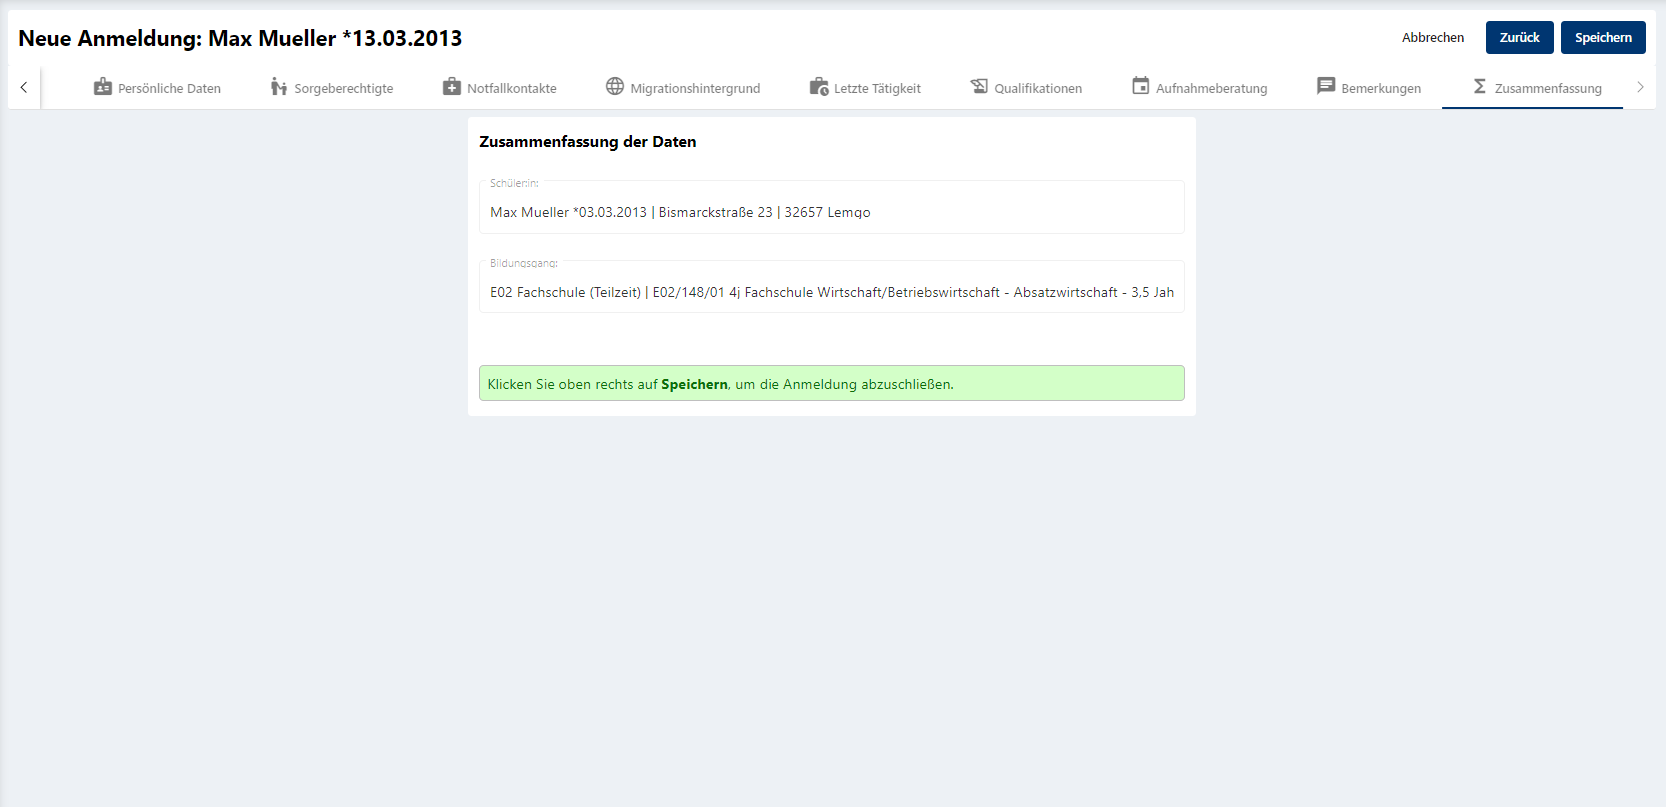
\includegraphics{zusammenfassung}
    \end{adjustbox}
\end{figure}

\subsection{bestaetigung}
\begin{figure}[H]
    \centering
    \caption{Testüberschrift}
    \begin{adjustbox}{width=\linewidth, center}
        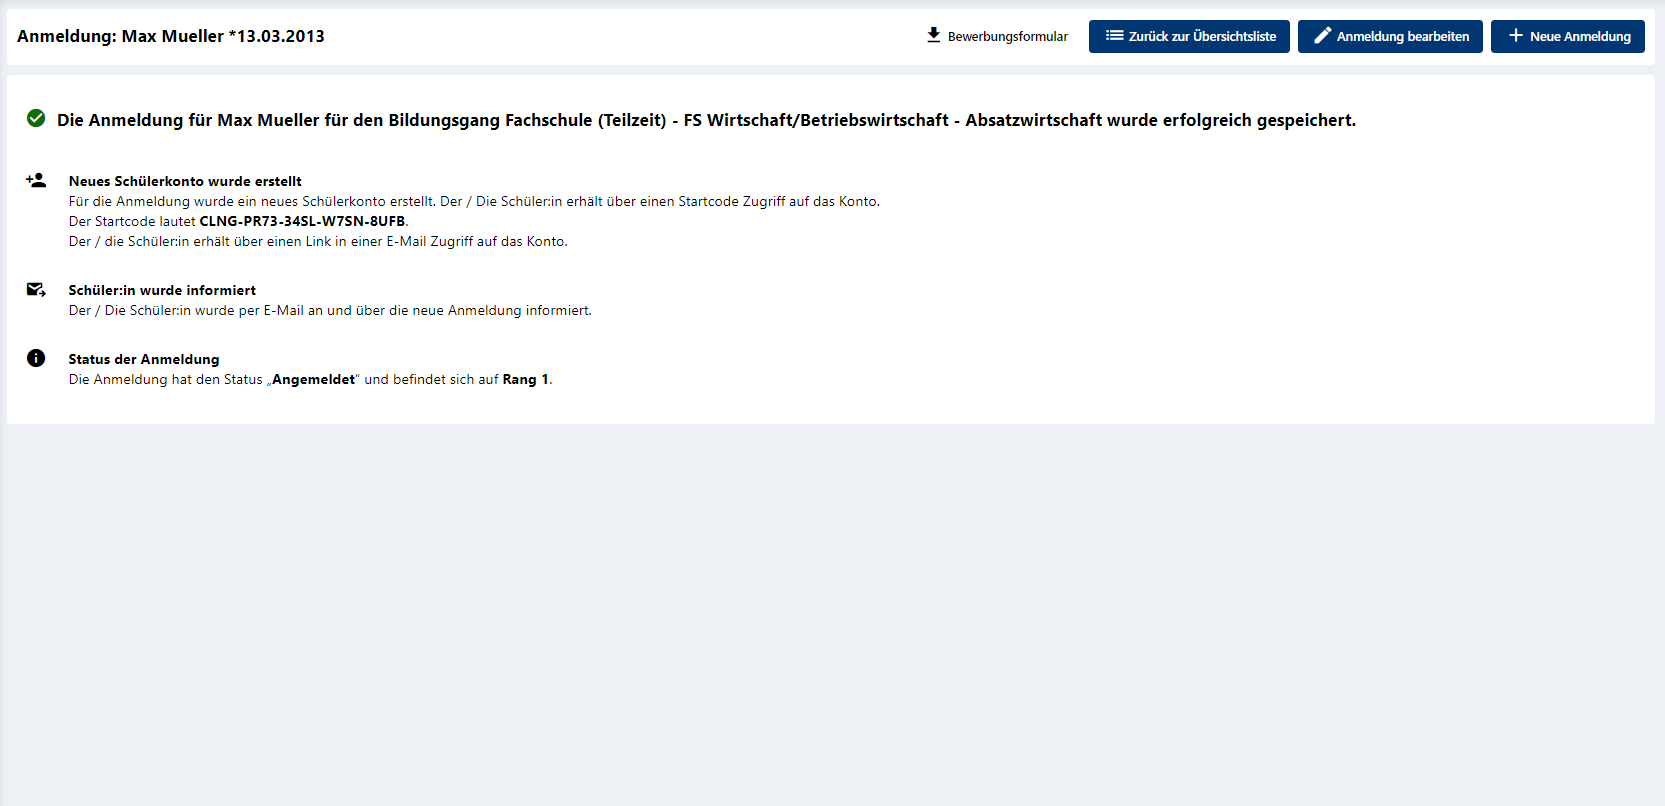
\includegraphics{bestaetigung}
    \end{adjustbox}
\end{figure}

\subsection{update-bewerbung}
\begin{figure}[H]
    \centering
    \caption{Testüberschrift}
    \begin{adjustbox}{width=\linewidth, center}
        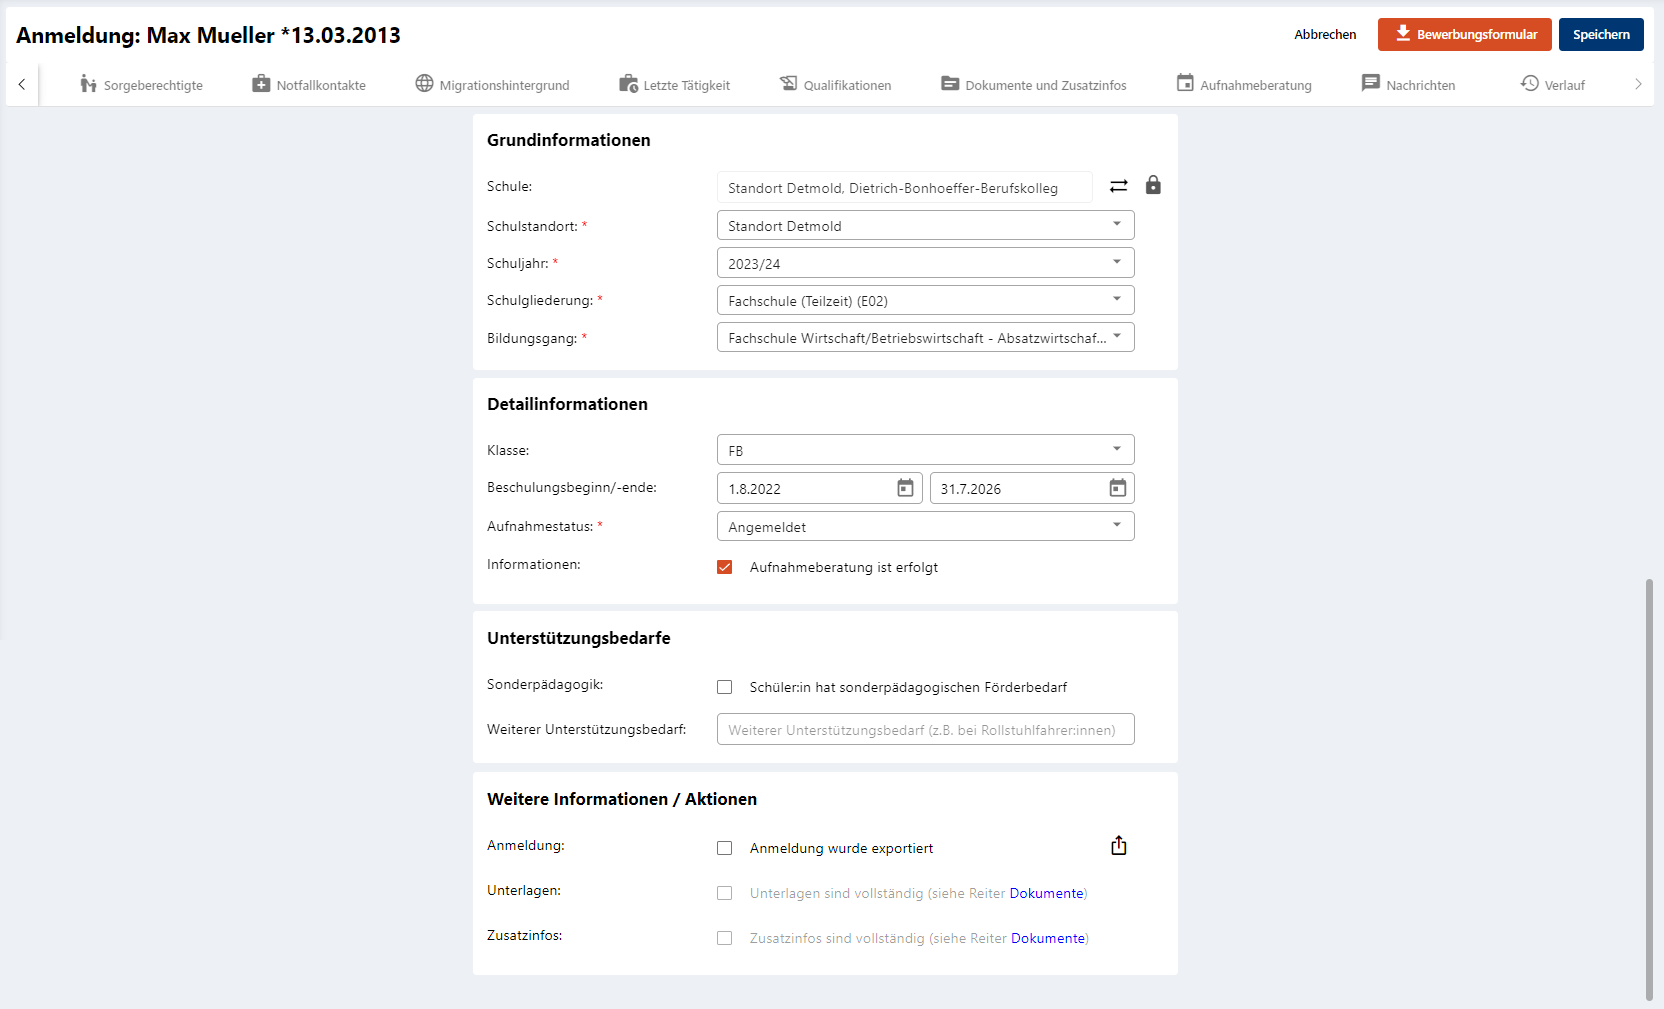
\includegraphics{update-bewerbung}
    \end{adjustbox}
\end{figure}

\end{landscape}
